\begin{figure*}[t]
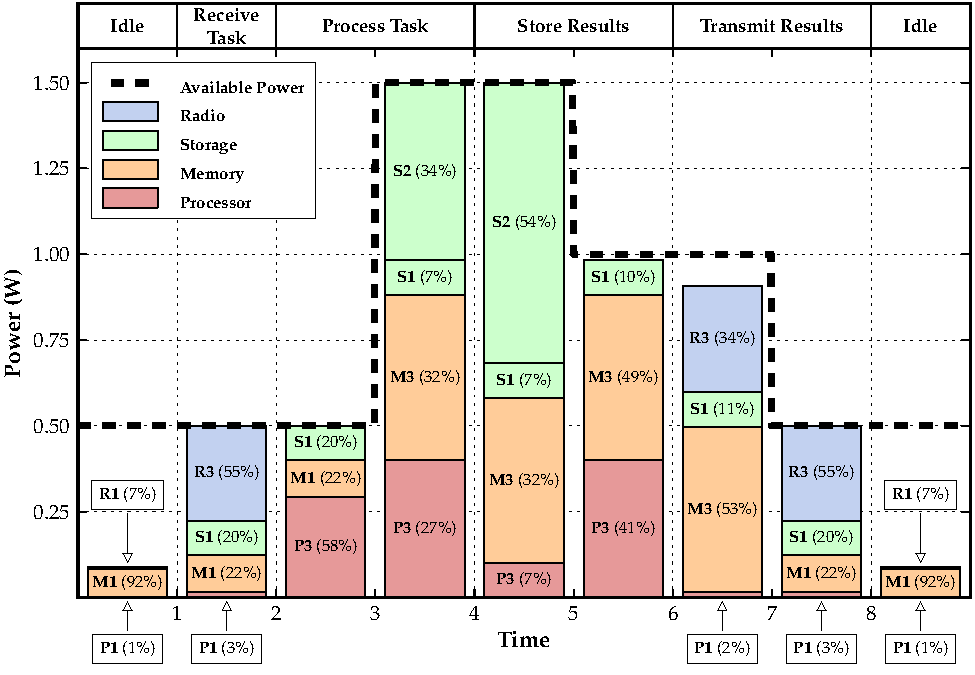
\includegraphics[width=\textwidth]{./figures/transitiongraph.pdf}
\noindent\begin{minipage}[t]{0.5\textwidth}
\vspace{-0.05in}
\begin{tabularx}{\columnwidth}{cX}

\textbf{0} & Awaiting tasks, \textbf{P1} and \textbf{M1} are idle, while
\textbf{R1} operates at low duty cycle.
\\

\textbf{1} & 
Alerted to an incoming task, the device activates \textbf{R2} to rapidly
receive task data and \textbf{S1} to store it.
\\

\textbf{2} &
When processing begins, energy usage is reconfigured by activating
\textbf{P2} and disabling \textbf{R2}.
\\

\textbf{3} &
When availability spikes processing is accelerated by activating \textbf{M2}
and mirroring to \textbf{S2}.
\\

\end{tabularx}

\end{minipage}
\begin{minipage}[t]{0.5\textwidth}
\vspace{-0.05in}

\begin{tabularx}{\columnwidth}{cX}

\textbf{4} &
As results start being written to disk, power usage shifts within the same
component ensemble.
\\

\textbf{5} & 
When availability drops to 1~W, the device stores compressed results on
\textbf{S1}.
\\

\textbf{6} &
To return results, \textbf{R2} is driven by \textbf{P1}.
\\

\textbf{7} &
When availability falls again, the device disables \textbf{M2} and
switches to the smaller memory chip \textbf{M1}.
\\

\textbf{8} &
Processing is complete.
\\

\end{tabularx}
\end{minipage}
\vspace{-0.1in}
\caption{\normalsize \XXXnote{GWA: TODO: Fixme.}}

\label{figure-transitiongraph}
\vspace{0.10in}
\hrule
\vspace{-0.20in}
\end{figure*}
